\chapter{Audio Signal Processing and Inverse Problem}\label{ch:processing}
\openepigraph{Sound, a certain movement of air.}{Aristotele, De Anima II.8 420b12}
\vspace{-2.5em}
\newthought{Synopsis} Let us now move from the physical domain to discrete time
signal processing
\blindtext[1]
Notation and definition are based on \cite{gannot2017consolidated}.

\section{Signal Model and Definitions}\label{sec:processing:model}
\marginpar{
    \footnotesize
    In this section and in the rest of the dissertation,
    we adopt the following general notations defined in~\cpageref{ch:notation}
    and introduced by \citeonly{gannot2017consolidated}.
}
In this thesis, an \textit{auditory} scene consists in sound \textit{sources}, \textit{microphones} deployed in a room.
The signals are emitted by sources and they are observed, received or recorded by microphones.
A set of microphones is called a microphone \textit{array} and its signal are called \textit{channels}.

Let us assume the observed signal has $\numMics$ \textit{channels} indexed by $\idxMic \in \kbrace{1,\dots,\numMics}$.
A \textit{single-channel} signal ($\numMics = 1$) is represented by the scalar $\mic(t) \in \bbR$,
while a \textit{multichannel} ($\numMics >   1$) is represented by the vector
$\mics(t) = \ktranspose{\klist{\mic_1(t), \dots, \mic_{\numMics}(t)}} \in \bbR^{\numMics \times 1}$.
The $\idxMic$-th microphone have a well defined position in the space which is denoted with $\positionMicrophone_\idxMic$.
\\Furthermore, let assume that there are $\numSrcs$ sources indexed by $\idxSrc \in \numSrcs$.
Sources can be of two types:
\begin{description}
    \item[Point sources] are emitted by a single and well-defined point in the space $\positionSource_\idxSrc$ and their signal is single channel.
    Point sources are for instance human speakers or the sound emitted by a loudspeaker.
    \item[Diffuse sources] refers for instance to wind, traffic noise, or large musical instruments, which emit sound in a large region of space.
    Their sound cannot be associate to a punctual source, but rather a distributed (infinite) collection of them.
\end{description}

\newthought{The Mixing Process} leading to the observed signal can be
using by means of an intermediate representation~\cite{sturmel2012linear}:
\begin{center}
    \textit{The \emph{source spatial images}, or \emph{images},  $\img_{\idxMic\idxSrc}(t)$ describes the contribution
    of the source $\idxSrc$ to the microphone $\idxMic$ by means of a spatialization
    operation\sidenote{\eg/ the propagation from the point source to the microphone including reverberation}}.
\end{center}
Being $\spat_\idxSrc(\cdot)$ a possibly nonlinear spatialization operation, the spatial images
$\imgs_\idxSrc(t) = \ktranspose{\klist{\img_{1\idxSrc}(t), \dots, \img_{\numMics\idxSrc}(t)}}$ with respect to the $\numMics$ reads
\begin{equation}
    \imgs_\idxSrc(t) = \kbracket{\spat_\idxSrc(\idxSrc)}(t)
    .
\end{equation}
In second stage, the images of all (point and diffuse) sources are added together and passed through a possibly
nonlinear \textit{post-mixing} operation $\master(\cdot)$ to obtain the mixture signal $\mics(t)$
\begin{equation}
    \mics(t) = \kbracket{ \master\kparen{
                    \sum_{\idxSrc=1}^{\numSrcs} \imgs_\idxSrc
                    }}(t)
\end{equation}
\marginpar{
    \footnotesize
    In the field of music productions,
    $\spat_\idxSrc(\cdot)$ and $\master(\cdot)$ may be identify rispectively with the \textit{mixing} and \textit{mastering} process.
}
\begin{figure}[t]
    \centering
    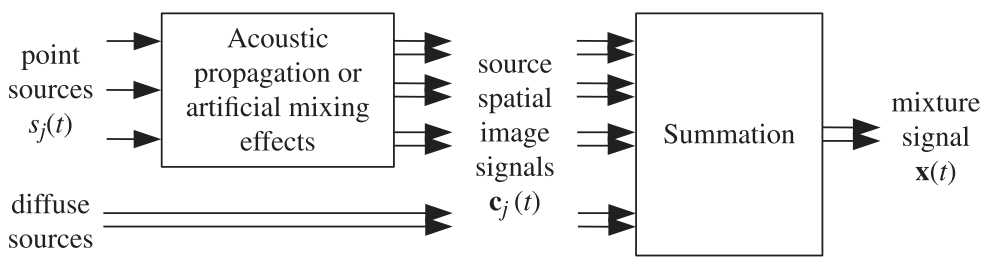
\includegraphics[width=\linewidth]{processing/mixing_process.png}
    \caption{General mixing process,
    illustrated in the case of $\numSrcs = 4$ sources,
    including three point sources and one diffuse source, and $\numMics = 2$ channels.}
    \label{fig:processing:mixing}
\end{figure}
\textsc{In Room Acoustics, the mixing process} is due to the propagation of sound in the auditory scene.
As discussed in~\cref{ch:acoustics:sec:wave}, this process is linear (and time invariant provided a static scenario).
In this case, the spatialization operation $\spat_\idxSrc(\cdot)$ is expressed by
collection of convolution with \RIR/ $h_{\idxMic\idxSrc}$
from source $\idxSrc$ to microphone $\idxMic$ and the post-mixing operation $\master(\cdot)$ reduces to the identity:
\begin{align}
    \img_{\idxMic\idxSrc}(t) &=  \kparen{h_{\idxMic\idxSrc} \conv \src_\idxSrc} (t) \\
    \imgs_\idxSrc(t) &=  \ktranspose{\klist{\img_{1\idxSrc}(t), \dots, \img_{\numMics\idxSrc}(t)}}\\
    \mics(t)         &= \sum_{\idxSrc=1}^{\numSrcs} \imgs_\idxSrc(t)
\end{align}
where $\conv$ is the linear convolution operator.
% \sum_{\tau=-\infty}^{+\infty} \bsh_\idxSrc(\tau) s_\idxSrc(t - \tau)

With the above notation, all the sources are threated in the same way, including \textit{target}, \textit{interfering} and \textit{noise} sources.
These definition depends on the specific use case, field of research and application.
Nevertheless, in speech processing context,
it is common to refers to interfering and noisy sources as undesired speech \vs/ nonspeech sources respectively.

%%%%%%%%%%%%%%%%%%%%%%%%%%%%%%%%
\section{Audio Inverse Problems}
\cite{kitic2015cosparse}
\openepigraph{Their generality is of such a wide scope that onemayeven argue that solving inverse problems is what signal processing is all about}{Srdan Kiti\'c, \textit{Cosparse regularization of physics-driven inverse problems}}
\openepigraph{everything is an optimization problem}{\citeonly{watson2001nonlinear}}
\marginpar{
    \footnotesize
    One can see the paralelism with the engineering concepts: analysis and sythesis.
}
In~\cref{sec:intro:problem} we have informally defined \textit{inverse problems}, with an emphasis on inverse problems in signal processing.
An inverse problem is a type of a mathematical problem where we start with the observations and we want to estimate model parameters that produced them.
\\Inverse problems pervades all the field of science and engineering:
source localization~\cite{},
image processing~\cite{},
acoustic imaging and tomography~\cite{},
\marginpar{
    \footnotesize
    A historical example are the calculation of the Earth circunference by Eratosthenes in III century b.c.\\
    and the calculations of Adams and Le Verrier which led to the discovery of Neptune from the perturbed trajectory of Uranus.
}

A inverse problems is defined as the counterpart of a \textit{forward}\sidenote{often referred to as \textit{direct}} problem.
Without falling in and deep mathematical formalism and taxonomies which can be found in \citeonly{bal2012introduction},
we will simply consider the following informal definition:
\begin{center}
    \textit{\emph{Forward problem} starts from known input, while \emph{inverse problem} starts from known output~\cite{santamarina2005discrete}.}
\end{center}
Both these problems focus on an operation relating maps objects of interest, called \textit{parameters} or \textit{variables},
to information collected about these objects, called \textit{measurements}, \textit{data} or \textit{observation}.

For instance, in our context, the direct problem may be the estimation of the \RIR/(s) starting from the known room parameters,
and, the related inverse problem would be the estimation of such room properties from the observation of the \RIR/(s).

Formally, a forward problem is defined through a mathematical model, described by a \textit{operation} $\scrM(\cdot)$
mapping \textit{parameters} $x \in \scrX$ to the \textit{observation} (or measurement) $y \in \scrY$:
\begin{equation}\label{eq:processing:model}
    y = \scrM(x)
    .
\end{equation}
Then, the inverse problem defines a method $\kinv{\scrM}$ that ``reverts'' $\scrM$ in order to recover (estimate) $x$ form the observation of $y$.
% The operator $\scrM$ describes our best effort to construct a \textit{model} for the available data $y$.
% The choice of $\scrX$ describes our best effort to characterize the space where we believe the parameters belong.

As discussed in~\cite{bal2012introduction}, \textit{solving} the inverse problem consists in finding point(s) $x \in \scrX$ from (knowledge of) data $y \in \scrY$
such that~\cref{eq:processing:model} or an approximation of~\cref{eq:processing:model} holds.
Under this light, the operator $\scrM$ ant the choice of $\scrX$ describes our best effort to construct a \textit{model} for the data $y$ and
the space where the parameters $x$ belong, respectively.
\marginpar{
    \footnotesize
    one can already see the paralelism the the definition of the mixing process defined in~\cref{sec:intro:problem}
}

\textsc{For instance, in Case of} \textit{linear} inverse problem, and for $\scrY$ and $\scrX$ being vector spaces of dimensions $M$ and $N$ respectively,
then the forward map can be written as a linear system:
\begin{equation}\label{eq:processing:linear_forward}
    \bfy = \bfM \bfx
\end{equation}
where $\bfM$ being a matrix, namely the operator $\scrM$ becomes a matrix multiplication by $M$.
It follows that the inverse map associated to~\cref{eq:processing:linear_forward} is the application of the inverse matrix $\kinv{M}$.
% While solving a direct problem the an operator needs to be found, in solving the inverse one either the operator is known and needs
% to be $reverts$t

Typically, forward problems are considered somehow the ``easier''.
In fact, even in the observation model $\scrM$ is known perfectly, it is not always possible to find its counterpart.
This because of
\begin{itemize}
    \item presence of \textit{noise} in the measurement which are not always additive and statistically independent \wrt/ $x$.
    \item the problem is \textit{well-posed} and \textit{well-conditioned}, namely $\scrM$ needs be injective and stable.
    In other words, some information is recoverable, other is completely lost, other highly sensible to noise
    \sidenote{
        \textbf{injective} ensure the uniqueness of the solution, while \textbf{stability}
        ensure a continuity on the data.
        These are known as the Hadamard's \textit{solvability conditions}.
    }.
\end{itemize}

As we could images, many interesting and fundamental inverse problem are
\textit{ill-posed} or \textit{ill-conditioned} in general, even in the following ``simple'' ones~\cite{kitic2015cosparse}:
The solution to the deconvolution problem, where the direct inversion of the transfer function results in instabilities
at high frequency; and the solution a linear system $\bfy = \bfM \bfx$ where $\bfM$ is invertible
may lead to erroneous results and numerical instabilities.

Therefore, sometimes ones have to settle for restring the set of solution $\scrC \subset \scrX$,
where $\scrM$ is stable and injective\sidenote{This framework was originally proposed by Tikhonov.}.
Promoting solution $x \in \scrC$ is can be achieved through \textit{model priors}, namely prior knowledge about solution, which can
be classified in the following methodologies:
the usage of \textit{geometric constraints} that deterministically define the solutions; the imposition of \textit{penalization}
which ``promotes'' solution of a certain shape (\eg/ \textit{sparse}
\sidenote{\textbf{sparsity} is a fundamental concept of this thesis, better discussed in~\cref{pt:estimation}
} or \textit{smoothness});
and casting the problem in a \textit{bayesian framework} which versatilely incorporate prior and posterior density function describing the data.

\subsection{General Processing Scheme}
Digital signal processing (DSP) is the process of analyzing and modifying a signal to optimize or improve its efficiency or performance. It involves applying various mathematical and computational algorithms to analog and digital signals to produce a signal that's of higher quality than the original signal.
It is traditional in engineering to represent complex systems as a collection of simpler subsystems, with well-defined tasks, interacting with each other.
In signal processing, these subsystems roughly fall into four categories: \textit{representation}, \textit{enhancement}, \textit{estimation}, and \textit{adaptive processing}.
Many problems can be decomposed into blocks that belong to one of these categories.

\begin{description}
    \item[Representation] Objects can be represent (described) in many different way.
    Through different representations, some object \textit{information} becomes more relevant and suitable for certain tasks
    than other.
    \\Representation can be lossy or lossless, and are generally implemented through (non)linear mapping, such as change of basis or feature.
    The most famous representation is the Fourier basis.
    \\Depending on the task the representation may be invertible.
    \\Analysis and Synthesis

    \item[Enhancement] Measurement are affected by noise and interferences which corrupt and hide relevant information, making inverse problems ill-posed and ill-conditioned.
    Therefore, signal enhancement, that is removing noise, is a necessary step.
    \\Enhancement constitute a huge dome of methods: form simple denoising by averaging of repeated measurement to
    spectral subtraction to source separation with neural network.

    \item[Estimation] Often we wish to estimate some key properties of the target signal which may be used as inputs to a different algorithm.

    \item[Adaptive processing] deals with adaptive algorithms and filters controlled by variable parameters.
    A common means to adjust those parameters according to an optimization algorithm which rely on statistical properties of the signal of interest.
    They often implement a kind of online optimization where an objective function is being minimized.
    When new data is observed, its discrepancy with the current estimate is used to produce a new estimate in a way that reduces the objective.
\end{description}

Let us give two example of practical systems that will be recurrent thought out the entire thesis.

\subsection{Selected Audio Inverse Problems}
Here follow some famous problems in the field of audio signal processing with application to speech, music and environmental audio.
Given the mixing process defined in~\cref{sec:processing:model},

% \begin{description}
%     \item[sound source separation and enhancements] as the problem of retrieving a (set of) source signal from a mixture.
%     \item[sound source localization] estimation of source location from the observation of the sound production.
%     This has sense as long as the impulse response convey space properties.
%     \item[microphones calibration] estimation of the microphone placement.
%     \item[\RIR/ estimation] estimation of the filters.
%     Blind Channel Estimation or System Identification.
%     \item[Acoustic Echoes Estimation] estimation of the filters
%     \item[dereverberation] estimation of the filters
%     \item[room geometry estimation] estimation of the room
%     \item[automatich speech recognition]
% \end{description}

\begin{table}[!h]

    \begin{fullwidthfig}
    \centering
    \small

    \begin{tabular}{p{0.33\linewidth}|p{0.66\linewidth}}
        \toprule
        Inverse Problem & \textit{Can we estimate the...} \\
        \hline
        Audio Source Separation  & the signal of the sources $s_{j}$ from the mixture $\boldsymbol{x}$? \\

        Sound Source Localization & the position $\mathbf{s}_{j} \ =\ [ x_{s_{j}} ,\ y_{s_{j}} ,\ z_{s_{j}}]$  of the source $s_{j}$ from the mixture $\boldsymbol{x}$$ $? \\

        Microphone (Array) Calibration & the position of the microphone (array) position $\mathbf{x}$ from the mixture $\boldsymbol{x}$? \\

        \RIR/ Estimation & the filter between the sources $\boldsymbol{s}_{j}$ and the mixture $\boldsymbol{x}$ from $\boldsymbol{x}$? \\

        Room Geometry Estimation & the shape of the room in which the mixture $\boldsymbol{x}$ recoding source $s_{j}$? \\
        \bottomrule
    \end{tabular}

    \end{fullwidthfig}

    \vspace{-\baselineskip}\vspace{-\baselineskip}
    \sideparmargin{outer}
    \sidepar{\vspace{\baselineskip}
        \caption{Selected audio inverse problems}
    }
    \label{tab:processing:problems}


\end{table}

\openepigraph{Everything is connected}{Douglas Adams, \textit{Dirk Gently's Holistic Detective Agency}}
\newthought{Depending on the scenario}, all these problems exhibits strong inter-connections,
namely the solution of one may be (dependent on) the solution of another.
Therefore, exploiting expertise and knowledge,
interconnect and hierarchical approaches may be built\sidenote{Machine Learing allows now for end2end approaches}:
for instance, many spatial filtering techniques used for \SE/ rely on \SSL/ blocks;
and in order to achieves \RooGE/, \AER/ must be done.

\section{Time, Frequency and Time-Frequency}
\subsection{Time and Frequency}

\subsection{Time-Frequency Analysis Synthesis}

\subsection{Time-Frequency Filtering}

% \section{Evaluation of an Inverse Problem}
% The inverse problem above listed are far to be solved or solved in everyday-life conditions.
% Ground-truth parameters

%%%%%%%%%%%%%%%%%%%%%%%%%%%%%%%%
\section{Taxonomy through dichotomies}
%% acoustics %%
\newthoughtpar{Source \vs/ Mixtures}
\newthoughtpar{Single-Channel \vs/ Multichannel}
\newthoughtpar{Point \vs/ Diffuse Sources}
\newthoughtpar{Directonal \vs/ Onmidirectional Recordings}
\newthoughtpar{Diffuse \vs/ Measurements Noise}
%% processing %%
\newthoughtpar{Speech \vs/ Music processing}
\newthoughtpar{Instantaneous \vs/ Convolutive Mixtures}
\newthoughtpar{Natural \vs/ Artificial Mixtures}
\newthoughtpar{Linear \vs/ Nonlinear}
%% pipeline %%
\newthoughtpar{Problem \vs/ Model}
\newthoughtpar{Synthesis \vs/ Abstaction}
%% problems %%
\newthoughtpar{Separation \vs/ Enhancement}
%% models %%
\newthoughtpar{end2end \vs/ 2step}
end2end: from data to (feature to) target
\\2-step: (from data to features) + features to target

\newthoughtpar{Knowledge-based \vs/ Learning-based}
\begin{itemize}
    \item Bottom-up vs Top-down information processing
    \item Knowledge-based: specialized signal processing and mathematical algorithms informed by knowledge;
    \item Learning-based: machine learning usually trained in supervised fashion.
\end{itemize}

\newthoughtpar{Supervised \vs/ Unsupervised}
\newthoughtpar{Machine Learning \vs/ Deep Learning}

\section{Time-Frequency Analysis and Synthesis}

\subsection{Artificial Mixtures}

\subsection{Impulse Response Models}
\newthoughtpar{Acoustic and Room Impulse Response}

\newthoughtpar{Acoustic and Room Transfer Functions}

\newthoughtpar{Steering Vectors}

\newthoughtpar{Relative Transfer Functions}

\newthoughtpar{Full-Rank Covariance Models}
